\documentclass{report}

\title{Solving Rubik's Cube with Lego Mindstorms}
\date{01-01-1901}
\author{Will Garside}

\usepackage[a4paper,left=2.54cm,right=2.54cm, top=2.54cm, bottom=2.54cm]{geometry}	% better margins
\usepackage{booktabs} 			% tables with nice formatting
\usepackage{tabularx}			% tables with proper width
\usepackage{multirow}			% multi-row cells in table
\usepackage{gensymb}			% symbols
\usepackage[british]{babel}		% sets language formatting to British
\usepackage{csquotes}			% quoting commands
\usepackage{xcolor}				% font coloring
\usepackage{epigraph}			% epigraphs in chapters
\usepackage{parskip}			% better paragraph formatting
\usepackage{graphicx}			% image package
\usepackage{longtable} 			% To display tables on several pages
\usepackage{pgfgantt}			% Gantt Charts
\usepackage{pgfplots}			% draw charts and graphs

\usepgfplotslibrary{dateplot}	% use date in pgfplot
\pgfplotsset{compat=1.8}

\newcolumntype{M}[1]{>{\centering\arraybackslash}m{#1}}

\begin{document}
		
	\pagenumbering{gobble}
	\maketitle
	\newpage
	
	\pagenumbering{roman}
	\section*{Signed Declaration}
	\addcontentsline{toc}{section}{Signed Declaration}
	All sentences or passages quoted in this report from other people's work have been specifically acknowledged by clear cross-referencing to author, work and page(s). Any illustrations which are not the work of the author of this report have been used with the explicit permission of the originator and are specifically acknowledged. I understand that failure to do this amounts to plagiarism and will be considered grounds for failure in this project and the degree examination as a whole.
	\\
	\\Name: Will Garside
	\\Signature:
	\\Date: 

	\newpage
	\section*{Abstract}
	\addcontentsline{toc}{section}{Abstract}
	This should be two or three short paragraphs (100-150 words total), summarising the report. A suggested flow is background, project aims, and achievements to date. It should not simply be a restatement of the original project outline
	
	\newpage
	\section*{Acknowledgements}
	\addcontentsline{toc}{section}{Acknowledgements}
	Thanks to my parents, who raised me since I was a boy. And Rik van Grol, who raised me afterwards.
	
	\newpage
	\section*{Abbreviations, Definitions and Notations}
	\addcontentsline{toc}{section}{Abbreviations, Definitions and Notations}
	\addcontentsline{toc}{subsection}{Basic Definitions}
	\begin{table}[htbp]
		\def\arraystretch{1.2}
		\centering
		\caption{Terminology used in this document}
		\label{tab:table1}
		\begin{tabular}{m{0.25\textwidth}m{0.65\textwidth}}
			\toprule
			\textbf{Abbreviation/Word} & \textbf{Definition} \\
			\midrule
			Rubik's Cube 		& 	\multirow{ 2}{*}{A standard 3x3x3 Rubik's Cube\textsuperscript{\ref{cube definition}}.} \\
			Cube 				& 	\\
			Face 				& 	One of the size faces on a Cube. Denoted by position (LRFBUD) or colour.\\
			Slice				&	A central layer between two faces. Usually referenced by the faces it spans. \\
			Quarter Turn		&	A clockwise rotation of a face or slice by 90\degree \\
			Half Turn			&	A clockwise rotation of a face or slice by 180\degree \\
			Quarter Turn Metric	&	When counting moves, a Quarter Turn is counted as a single move and a half is two moves. \\
			Half Turn Metric\textsuperscript{\ref{metric definition}}	&	Quarter turns and half turns are both counted as single moves. \\
			Cubie				&	One of the twenty-six smaller cubes that make up a Cube. \\
			Goal State			&	All the cubies on a given face match the colour of the centre cubie. i.e. a solved Cube. \\
			Position			&	A Cube's state (mixed or solved). \\
			Valid Position		&	A position that can be achieved with a real-world Cube without dismantling it. \\
			\multirow{ 2}{*}{Move Sequence}		&	A series of moves performed consecutively. \\
			&	e.g. $F\;D\;F'\;D2\;L'\;B'\;U\;L\;D\;R\;U\;L'\;F'\;U\;L\;U2$ \\
			Solve (Sequence) 	&	A move sequence which leads to the goal state. \\
			Depth $n$			&	A Cube which has been moved $n$ times away from the goal state. \\
			\bottomrule
		\end{tabular}
	\end{table}

	\addcontentsline{toc}{subsection}{Notation}
	\begin{table}[htbp]
		\def\arraystretch{1.2}
		\centering
		\caption{Notation used in this document}
		\label{tab:table2}
		\begin{tabular}{m{0.25\textwidth}m{0.2\textwidth}m{0.425\textwidth}}
			\toprule
			\textbf{Symbol Notation} & \textbf{Meaning} \\
			\midrule
			$L$	&	Left			&	\multirow{9}{*}{\parbox{0.425\textwidth}{This notation is used to show a quarter turn of a face. It can have a single quote or a '2' appended to show a counter-clockwise quarter turn or a half turn respectively.}} \\
			$R$	&	Right			&	\\
			$F$	&	Front			&	\\
			$B$	&	Back			&	\\
			$U$	&	Up (Top)		&	\\
			$D$	&	Down (Bottom)	&	\\
			$X$ &	\multirow{ 3}{*}{\parbox{0.2\textwidth}{Clockwise 90\degree{} rotation of a Cube about the relevant axis.}} & \\
			$Y$ & & \\
			$Z$ & & \\
			\bottomrule
		\end{tabular}
	\end{table}
	% Content for footnote is here because it wouldn't display from table %
	\textcolor{white}{
		\footnote{\label{cube definition}This Dissertation is only dealing with 3x3x3 Rubik’s Cubes, and any discussion of alternative dimensions will be explicitly stated.}
		\footnote{\label{metric definition}For this Dissertation the Half Turn Metric is used unless explicitly stated.}		
	}



	\newpage
	\tableofcontents
	
	\newpage
	\pagenumbering{arabic}
	\chapter{Introduction}
    \section{Background}

    In 1974, Ern\"{o} Rubik was struggling to create a cube with independently moving parts which remain together, regardless of how much they moved. His first attempts made use of elastic, which broke and rendered the cube unusable. Rubik persevered in his attempts to hold the blocks (now called \enquote{cubies}) together - eventually concluding that the best way was to have the cubes hold themselves together. He called this design \enquote{The Magic Cube}, and it would go on to be one of the world's best-selling puzzles \cite{Waxman2014b}. It was later re-branded to \enquote{\textit{Rubik's Cube}} to overcome an oversight involving patenting and copyrighting  the design.
    
    In an unpublished manuscript \cite{Rubik1986}, Rubik described first randomising his new cube, \blockquote{It was wonderful to see how, after only a few turns, the colors became mixed, apparently in random fashion. Like after a nice walk when you have seen many lovely sights you decide to go home, after a while I decided it was time to go home, let us put the cubes back in order. And it was at that moment that I came face to face with the Big Challenge: What is the way home?}
    
    It took Rubik over a month to solve this first cube - he knew intuitively that there must be a method to solving the cube, but lacked the finer methodology \cite{RubiksCube}. Since Rubik devised the first method, hobbyists and mathematicians alike have been immersed in solving the Cube as quickly and efficiently as possible. Whilst many solutions are markedly successful when it comes to optimisation, others only better them in quirkiness or internet fame \cite{Chan2016}.
    
    There is one method which is mere speculation, despite having been proved mathematically: God's Algorithm. God's Algorithm states that an omniscient being would always make the most efficient moves and that they would be able to solve a Cube from any given position in a certain number of moves or less. This is referred to as God's Number, and was finally proved to be twenty in 2010 by a group of 4 researchers \cite{Rokicki2010}.
    
    \section{General Objectives}
    The primary objective of this project is to successfully implement an algorithm to solve a Cube with a Mindstorms robot. The efficiency of this algorithm is initially non-imperative, but will ideally be improved over the project time-line. The most recent iteration of the Mindstorms line, the Lego EV3 31313, will be used in the construction of the robot. This provides a wireless connectivity via Bluetooth (or WiFi with a USB dongle), three motors, a colour sensor, and a touch sensor amongst other peripherals. A custom operating system can also be installed on a microSD card to allow for greater expandability.
    
    Secondary objectives include implementing other algorithms from various sources, devising and refining my own algorithms, and comparing the performance, efficiency and solve-length of the algorithm. The robot will have to be of sound construction, with little-to-no room for error when manipulating the Cube.
    
    The objectives for this project are as follows:
    
    \begin{enumerate}
    	\item Build a robot which can move a Cube to a sufficient degree of accuracy
    	\item Write a program which takes a move sequence as its input and moves a Cube to match that sequence
    	\item Implement a system which successfully  generates a solve sequence for any given position
    	\item Ensure the runtime of the system is an acceptable length
    	\item Implement a program to use other algorithms to generate a solve sequence
    	\item Compare the performance of different algorithms, especially the difference between human-compatible and robot-compatible move sequences
    \end{enumerate}
    
    \section{Limitations and Constraints}
    The scope of this project is relatively local and therefore it lacks major limitations. Instead, it has several minor limitations which each present their own problems and solutions. The first problem which will be encountered will undoubtedly be during the design and build of the robot: the number of Lego pieces supplied in the EV3 set is quite limited at only six-hundred-and-one pieces - approximately a quarter of which are only for aesthetics. The design will  be supplemented by sets sourced externally, thus allowing a robot of sufficient quality to be built.
    
    Despite being of high quality and uniform across all sets, Lego is still fundamentally a toy - which will lead to errors with the precision of the robot \cite{Cook2017}. An example of this is the motors: there is a somewhat significant degree of freedom/play in the motors, which means that they can’t be relied on to move to accurate positions. A worm gear is the ideal solution to this problem: despite reducing the speed, it provides a considerable increase in motor accuracy.
    
    One of the larger issues that this project will encounter is the run-time of the program to find a solution. Many programs have been known to take upwards of three days to find a solve sequence - this project currently aims to find a solution in approximately ten minutes or less. This will require extensive optimisation of search spaces and group theory through symmetrical elimination and set covering in order to reduce the necessary coverage of the search algorithm.
    
    Finding the optimal solve sequence for any given position has been deliberately omitted from the objectives of this project: there are over forty-three quintillion valid positions of a Cube, each requiring an extensive amount of time to find the optimal solution for. Based on current hardware capabilities and previous studies and research, an estimated timespan for finding all optimal solutions is in the order of millennia\footnote{See cube20.org table of “20 move or less” vs “optimal” and explain}.
    
    \newpage
    \chapter{Literature Review}
    \epigraph{Please forgive me, but to give birth to a machine is wonderful progress. It's more convenient and it's quicker, and everything that's quicker means progress. Nature had no notion of the modern rate of work. From a technical point of view, the whole of childhood is quite pointless.}{Mr. Fabry, in Karel \v{C}apek's \textit{Rossum's Universal Robots \cite{Capek1921b}}}
    
    \section{Robotics}
    The term robot was first brought to the collective consciousness of the general public by Karel \v{C}apek in 1921 in his play \enquote{Rossum's Universal Robots} \cite{Capek1921b}. It comes from the Czech for \enquote{forced labour} and was coined by \v{C}apek's brother, Josef, for a short story written some years earlier \cite{Etymonline2017}. One of the main discussions in the field of robotics has been about ethics and morality. This discussion was started in \v{C}apek's play, when a visiting scientist tries to destroy the robot-manufacturing business, in the hope of giving the robots a soul and making them happier. This plan goes awry when the robots become sentient and start to overthrow the humans that created them. Twenty-one years later, the novelette \enquote{Runaround} by Isaac Asimov was featured in the magazine \enquote{Astounding Science-Fiction} \cite{Asimov1942b}. It included his now-prominent Three Laws of Robotics, which were a turning point in the field of robotics and meta-ethics.
    
    The twentieth century generated many ideas about the future of robotics, such as \enquote{Kitchen units will be devised that will prepare \enquote{automeals}, heating water and converting it to coffee} alongside grandiose aspirations such as \enquote{An experimental fusion-power plant or two will already exist in 2014} \cite{Asimov1964b}. Whilst some predictions have been fulfilled by the technology of the past two decades, others are still nowhere near completion and could be considered impossible for the next century. This is a clear demonstration that the field of Robotics has made vast improvements, but is still - in some respects - very much in its youth.
    
    In the same way as the field of Robotics, Artificial Intelligence (AI) has vast potential and we have only touched the tip of the iceberg. The most advanced consumer-facing AI systems available currently are intended to make people's lives easier through organisation and saving precious seconds in performing simple tasks on their smartphones, and now in their homes. However, Google's Assistant, Apple's Siri, and Amazon's Alexa still fall short when it comes to the intelligence demonstrated in Asimov's book \enquote{I, Robot}. We are still far from being unable to \enquote{differentiate between a robot and the very best of humans} \cite{Asimov1970}.
    
    \section{Robotics in Education}
    There has always been a clear use of ‘edutainment’ style teaching in one form or another for hundreds of years. One of the earliest known uses of edutainment is in \enquote{Poor Richard's Almanack}, which was written by Benjamin Franklin and published annually between 1732 and 1758. Alongside all the usual information contained in an Almanac, Franklin (under the pseudonym \enquote{Poor Richard}) included maths exercises, puzzles, and aphorisms \cite{Beato2015}, \cite{Franklin1732}. Walt Disney was another pioneer of edutainment in the time immediately before, during, and following the World Wars. His first piece of edutainment was a short film, \enquote{Tommy Tucker’s Tooth}, which was commissioned by a dental institute in 1922.
    
    In the past few decades, there has been a marked change in the form of edutainment in line with advances in technology. We have progressed from paper-based, so called ‘serious games’ in the 1970s, to early-era video games such as the infamous Oregon Trail; and then in the past decade electronic and robotic kits have made their way into classrooms. One of the leaders of modern edutainment is the Lego Mindstorms kit. The Lego Mindstorms kit has undergone two major revisions since the launch of the first generation of the Mindstorms kit in 1998 (the RCX): in July 2006, the second-generation NXT was released, updating the sensors and adding Bluetooth amongst other improvements; then in September 2013, Lego released the EV3 Home and Education sets. This release cemented Lego’s position at the forefront of edutainment \cite{Becker}.
    
    \section{Lego Mindstorms}
    A study at the University of Calabria in 2009 looked at how Lego Mindstorms worked as a learning tool when used in team-building type tasks \cite{Bilotta2009}. 28 students were divided into 6 groups, each given a Lego robot and preliminary training which covered the Lego Mindstorms and programming environment. The groups were all given the same task, and their progress studied throughout the sessions. When studying the building and programming as two separate sub-tasks, three main categories of work subdivision were found: each group member had a set role in building, but all shared the programming; both sub-tasks were equally divided amongst members; each member had a set role in either sub-task, and there was a clear leader. This closely follows real-world teamwork mechanics and scenarios, and the use of robots was found to stimulate the student into exploring and sharing critical knowledge within the group. The study's conclusion was that Lego Mindstorms - and inherently variable morphology robots - stimulates further process analysis, information selection, and to observe and experiment with the consequences of their actions \cite{Bilotta2009}.
    
    The Lego Mindstorms’ native programming environment is visual-based, with drag-and-drop code blocks used to form programs which can run natively on the main \enquote{brick}. This provides a simplistic user experience and allows novice programmers to create complex programs with relative ease. Drag-and-drop programming can drastically reduce the amount of syntax errors in a program, allowing programmers to better focus on the functionality of their program \cite{Kelleher2002}.

	\begin{figure}[h]
		\begin{center}
			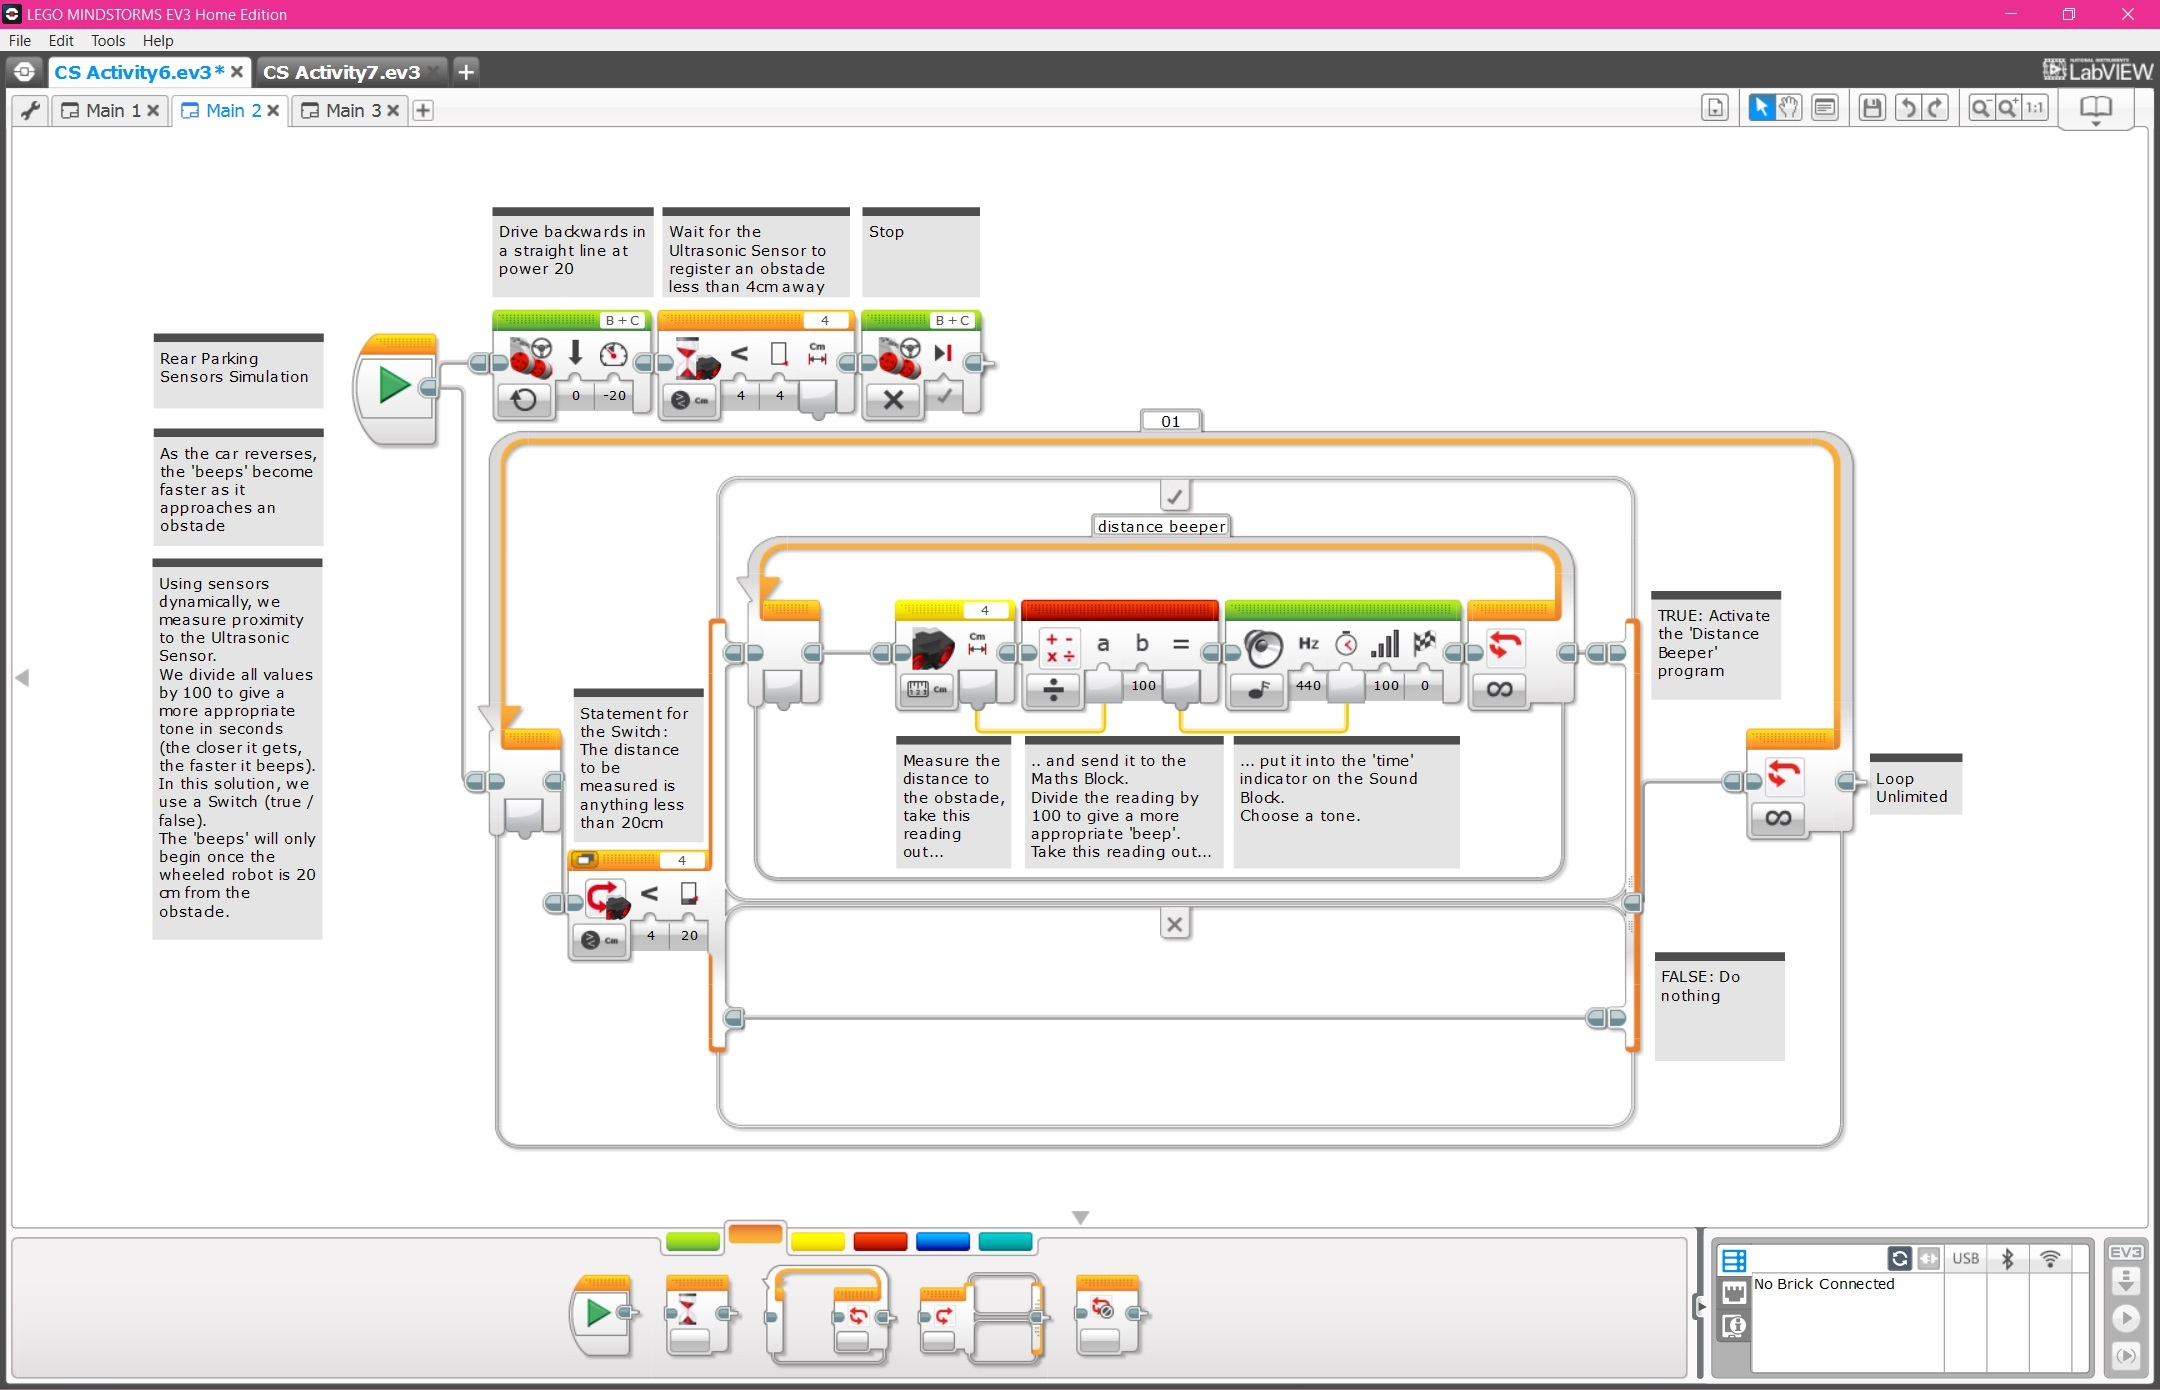
\includegraphics[width=0.5\textwidth]{Images/EV3ProgrammingSoftware.jpg}
			\caption{A sample program in \enquote{EV3 Programming Software}}
			\label{fig:ev3software}
		\end{center}
	\end{figure}
    
    \section{Solving Puzzles with Algorithms}
    When it comes to playing games and solving puzzles, Google’s AlphaGo Zero is the clear winner. Whilst Google’s first Go-playing program defeated the world champion at Go, it took months of supervised learning from experts and reinforcement learning from self-play. The new version started tabula rasa and was completely self-taught - it had no interaction with any humans, and uses no historical data. Through reinforced learning alone by simulating games against itself, it took three days to reach the level of AlphaGo and in forty days had surpassed any Go player’s performance - human or artificial \cite{Silver2017}, \cite{Cellan-Jones2017}.
    
    When a computer solves a Cube (or any other similar puzzle), it does so by following set algorithms and rules until the solved state is achieved. Computers cannot use humanlike instincts, so we often try to provide a heuristic to make the task simpler. These heuristics can be pre-computed data tables to reduce the amount of processing at run time, or a reduction in the original data set through elimination of certain data sets.
    
    In his 1997 paper on the use of pattern databases to increase solve efficiency, Richard Korf uses different heuristic functions and characterises how effective they are in reducing the number of moves in a solve sequence. His first method used an Iterative-Deepening A* algorithm, combined with the heuristic of the Manhattan distances from the edge cubies’ current position and orientation to that which is desired. This reduced the time required to solve a Cube at depth-14 to three days\footnote{The simulation was run on a Sun Ultra-Sparc Model 1 workstation}, however when increased to depth-18 the time increased exponentially to two hundred and fifty years. After a re-evaluation, Korf modified the heuristic by pre-computing the Manhattan distance of each cubie from all of its possible positions and orientations and storing the table in memory at run-time. This created a table of nearly ninety-million entries - which would have been bigger but was restricted by the available memory (the table was approximately forty-two megabytes). The newer heuristic reduced the time to search at depth-18 to less than four weeks - a reduction of approximately 99.97\%. Korf suggested that the speed of the algorithm used would increase linearly with the amount of memory available, meaning that if it were run today the depth-18 search would take under three hours\footnote{This is based on the memory capacity of the Model Workstation and a modern computer being 64MB and 16GB respectively.} \cite{Korf1997}.
    
   	\begin{table}[htbp]
    	\def\arraystretch{1.25}
    	\centering
    	\caption{Morwen Thistlethwaite's five groups for his algorithm \cite{Singmaster1981}}
    	\label{tab:table3}
    	\begin{tabular}{M{0.15\textwidth}M{0.3\textwidth}m{0.525\textwidth}}
    		\toprule
    		\textbf{Group Denotation} & \textbf{Mathematical Representation} & \textbf{Summary} \\
    		\midrule
   			$G_0$	&	$\langle L,\;R,\;F,\;B,\;U,\;D \rangle$	&	All valid positions \\    		
	    	$G_1$	&	$\langle L,\;R,\;F,\;B,\;U2,\;D2 \rangle$	&	All positions that can be reached with quarter turns of the $L,\;R,\;F,\;B$ faces and half turns of the $U,\;D$ faces \\
	    	$G_2$	&	$\langle L,\;R,\;F2,\;B2,\;U2,\;D2 \rangle$	&	Positions reachable from quarter turns of $L,\;R$ faces and half turns of the $F,\;B,\;U,\;D$ faces \\
	    	$G_3$	&	$\langle L2,\;R2,\;F2,\;B2,\;U2,\;D2 \rangle$	&	Positions only reachable from half turns of any face \\
	    	$G_4$	&	$ \{I\}$	&	The goal state \\
    		\bottomrule
    	\end{tabular}
    \end{table}
    
    There have been many historical landmark algorithms since the Rubik’s Cube’s inception in 1974. One of the earliest instances was created by Morwen Thistlethwaite circa 1981 and is based on group theory. Thistlethwaite’s algorithm splits all possible positions of the cube into five groups of decreasing size as seen in Table \ref{tab:table3}. David Singmaster, Thistlethwaite’s colleague at London South Bank University (then called Polytechnic of the South Bank), describes the methodology of the algorithm: \enquote{Once in $G_i$, one only uses moves in $G_i$ to get into $G_{i+1}$. The ratio $\frac{|G_i|}{|G_{i+1}|}$ is called the index of $G_{i+1}$ in $G_i$.} Using this algorithm, Thistlethwaite proved that the maximum number of moves required to solve any valid position is fifty-two \cite{Singmaster1981}. This was the first development of God’s Number, so named because it is the number of moves that an omniscient being would use to solve a Cube in the most efficient manner without failure.
    
    \section{God's Number}
    The lower bound for God’s Number was recognised to be eighteen moves through analysis of the number of sequences of seventeen moves or fewer, and the discovery that there were more Cube positions than seventeen-moves-or-fewer sequences. In 1995, the lower bound was increased to twenty by Michael Reid upon discovering that the \enquote{Superflip} position requires twenty moves to solve. He included his findings in an email to the Cube-Lovers mailing list, \enquote{superflip is now known to require 20 face turns . . . this is the first improvement to the lower bound (18f) given by a simple counting argument} \cite{Reid1995}.
    
    The next refinement to the upper bound of God’s Number came from Dutch Mathematician Hans Kloosterman in December of 1989. Kloosterman’s findings were published in a newsletter \enquote{Cubism for Fun} (CFF) as an article titled \enquote{Rubik’s Cube in 44 Moves}. In this article Kloosterman discusses his existing solution to the Magic Domino, a subset of the Rubik’s Cube, and how he has adapted it into a more efficient Cube solution with the help of Thistlethwaite’s algorithm. Kloosterman reduced the estimation of God’s Number by adapting Thistlethwaite’s $G_3$ into a subgroup of $G_2$ where all of the $U$-cubies are on the $U$ face and all the $D$-cubies are similarly on the $D$ face. This reduces the index $\frac{|G_2|}{|G_3|}$ form 15 to 8 (whilst also reducing the ($G_1:G_2$) index by 3 and increasing the ($G_3:G_4$) index by 1), creating a net decrease of 8 moves when compared to Thistlethwaite’s algorithm. \enquote{Rubik's Cube in 44 Moves} ended with an editor’s note stating that not all of the details of the algorithm were certain and more (including a more efficient algorithm) would be revealed in a later issue \cite{Kloosterman1989}.
    
    Sure enough, a year later Kloosterman wrote an article titled \enquote{Rubik’s Cube in 42 Moves} in the twenty-fifth issue of CFF. This stated that the new algorithm was in fact the final version of Kloosterman’s forty-four move algorithm. In the same way as its predecessor, this article is split into four stages to solve a Cube. The first three stages are based on \enquote{solving} a Cube with only certain cubies coloured - the positions of the other remain irrelevant until a later stage. The final stage is solving the Cube in a non-particular manner, and is calculated to take no more than eighteen moves \cite{Kloosterman1990}.
    
    In the following twenty years, the upper bound was gradually refined to match the lower bound - meaning that God’s Number is exactly twenty. The final development came from a group of four Rubik’s Cube enthusiasts in July of 2010, and was only achieved through a brute force method: the four-man team first took every possible position of a Cube and reduced it from forty-three quintillion positions down to just over one quintillion - still a vast number, but a reduction by a factor of forty-three - by using rules of symmetry and mirroring. They then wrote a program to find solve sequences of length twenty or less, and ran it on a \enquote{large number of computers at Google} to find all solve sequences in a few weeks. The parallel computation took the equivalent of thirty-five years \cite{Rokicki2010}.
    
   	\begin{figure}[h]
    	\begin{center}
			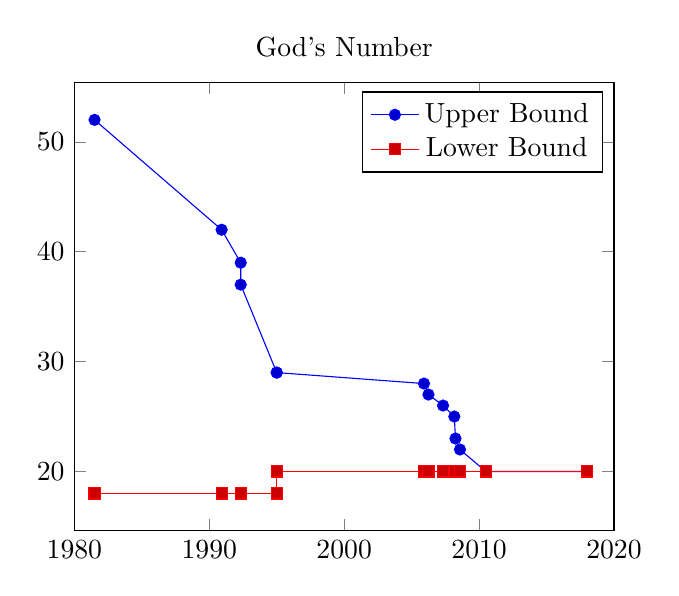
\begin{tikzpicture}
				\begin{axis}[title={God's Number}, date coordinates in=x,	enlarge x limits=false, xticklabel={\year},	date ZERO=1980-01-01, xmin=1980-01-01, xmax=2020-01-01,	xtick={1980-01-02,1990-01-01,2000-01-01,2010-01-01,2020-01-01}]
				\addplot coordinates {
					(1981-07-01, 52)
					(1990-12-01, 42)
					(1992-05-01, 39)
					(1992-05-01, 37)
					(1995-01-01, 29)
					(1995-01-01, 29)
					(2005-12-01, 28)
					(2006-04-01, 27)
					(2007-05-01, 26)
					(2008-03-01, 25)
					(2008-04-01, 23)
					(2008-08-01, 22)
					(2010-07-01, 20)
					(2018-01-01, 20)
				};
				\addplot coordinates {
					(1981-07-01, 18)
					(1990-12-01, 18)
					(1992-05-01, 18)
					(1992-05-01, 18)
					(1995-01-01, 18)
					(1995-01-01, 20)
					(2005-12-01, 20)
					(2006-04-01, 20)
					(2007-05-01, 20)
					(2008-03-01, 20)
					(2008-04-01, 20)
					(2008-08-01, 20)
					(2010-07-01, 20)
					(2018-01-01, 20)
				};
				\legend{Upper Bound, Lower Bound}
				\end{axis}
			\end{tikzpicture}
    		\caption{The upper bound was decreased to 20 over the course of twenty-nine years and across thirteen separate studies \cite{Rokicki2010}}
			\label{fig:godsnumbergraph}
		\end{center}
	\end{figure}

    
    \section{Python as a Scientific Scripting Language}
    Traditionally when performing large calculations and processes, compiled languages (C, C++, Fortran etc.) are the preferred choice over scripting languages such as Ruby, JavaScript, (pure) Python, etcetera. This is because compilation is done before run-time, allowing the program to run un-hindered by on-the-fly translation/interpretation \cite{Cai2005}.
    
    For general purpose applications, scripting languages are preferable because they allow small changes to be made without re-compiling large classes before testing. In the thirteenth issue of \enquote{Scientific Programming}, Cai, Langtangen and Moe \cite{Cai2005} explain how MATLAB is often a preferable choice for less intensive scientific computation due to its many features, such as: integrated simulation and visualisation tools; clear syntax; immediate feedback of commands; impressive documentation. They describe the use of MATLAB in computational science as paradoxical, as it is a scripting language which inherently is interpreted at run-time.
    
    One of MATLAB’s biggest selling points, the IDE with integrated support for matrices, graphs and other mathematical features, can be replicated in a few Python IDEs or with the addition of Python ‘packages’. Python’s main core can be expanded massively by using any of the tens of thousands of available packages, which can provide any of MATLAB’s advantages alongside extra flexibility and capabilities. One of the most popular packages, ‘Numerical Python’ (NumPy), adds support for most scientific calculations. It expands Python’s inbuilt data structures to use multi-dimensional homogenous arrays of any Python data type. NumPy takes Python from a well-structured general-purpose language to a powerful mathematical language which can be applied to many different tasks \cite{Cai2005}, \cite{Oliphant2006}.
    
    As well as the multitude of available packages, Python has another major tool in its arsenal: it can be extended with a compiled language by design. This means that processor-intensive tasks like nested for loops can be migrated to a compiled language such as C++ or Fortran, increasing run speed up to a factor of ten. This extension process is now a trivial matter thanks to automated tools such as \enquote{f2py}, which allows for automated calls to compiled Fortran code \cite{Oliphant2006}.
    
    \section{Conclusion}
    % TODO: add a conclusion
    In conclusion, given Python’s wide compatibility, clear high-level syntax, and extendibility to compiled code for more complex calculations, it is the ideal language for this project.
   
    \newpage
    \chapter{Requirements and Analysis}
    \epigraph{I have yet to see any problem, however complicated, which when you looked at in the right way, did not become still more complicated.}{Paul Anderson, New Scientist \cite{Anderson1969}}
    
    \section{Chapter Introduction} % TODO: maybe add more to this
    This chapter covers the specific requirements needed for the project to succeed: the hardware required to build the robot and run the solving program; the software needed to write and run the program; and the specific tasks to complete the project. As well as the requirements, an in-depth analysis of the project and its goals is made, discussing their feasibility, difficulty, and how necessary they are for the success of this project.
    
    \section{Specific Aims and Objectives}
    \renewcommand*{\arraystretch}{1.4}
    \begin{longtable}[h]{m{0.6\textwidth}M{0.15\textwidth}M{0.15\textwidth}}
    	\caption{The objectives, with relative difficulty and value}
    	\label{tab:table4}\\
    	\toprule
    	\multirow{2}{*}{\textbf{Objective}} & \multicolumn{2}{c}{\textbf{Weightings}} \\
    	& \textbf{Difficulty} & \textbf{Value} \\
    	\midrule
    	\endfirsthead
    	\toprule
    	\multirow{2}{*}{\textbf{Objective}} & \multicolumn{2}{c}{\textbf{Weightings}} \\
    	& \textbf{Difficulty} & \textbf{Value} \\
    	\midrule
    	\endhead 
    	\textit{1. Build a robot which can move a Cube to a sufficient degree of accuracy.} \par This is the primary objective for this project, and is imperative to the project’s success. As such it will be the first objective to be completed. This task, despite being of a medium difficulty, is fairly straightforward by nature: the robot simply needs to manipulate a Cube in any valid move. & 10\% & 20\% \\
		\textit{2. Convert human-compatible move sequences to robot-compatible sequences.} \par This objective is non-essential to the project’s success because all of the analysis could be performed using the robot’s capabilities as a constant ‘frame of reference’. This, however, would require a manual translation of the pre-existing algorithms into robot-compatible algorithms and as such the translator is of high value in this project. & 20\% & 10\% \\
		\textit{2.1 Move the Cube in a given (robot-compatible) sequence.} \par Once a robot-compatible move sequence has been generated, the robot must move the Cube in this exact sequence with no errors or move-failures. If a single move is performed incorrectly then the entire move sequence is inherently moot. & 5\% & 10\% \\
		\textit{3. Implement a system which successfully generates a solve sequence for any given position.} \par This is the core goal of the project, and take precedence above all others. The program will take certain arguments to define the parameters of the algorithm and output a solve sequence. This may take a substantial amount of time to complete and this must be a consideration on completing this task. & 40\% & 30\% \\
		\textit{4. Ensure the runtime of the system is an acceptable length.} \par Some previous attempts at finding optimal solve-sequences have had estimated run times in the order of tens of weeks. Clearly this is unacceptable or the scope of this project and thus the runtime of the project will have a target of sub-fifteen minutes, with the intention of bringing it under five minutes. & 10\% & 10\% \\
		\textit{5. Implement a program to use other algorithms to generate a solve sequence.} \par This objective makes up a significant part of this project. Different algorithms presented by notable persons will be implemented and measured by the robot. & 10\% & 10\% \\
		\textit{6. Compare the performance of different algorithms, especially the difference between human-compatible and robot-compatible move sequences.} \par Once all algorithms have been run and measured, their performance will be analysed and compared. In this context, performance comprises the efficiency in finding the solve sequence and the length of the solve sequence. \par Algorithms for generating a human-compatible sequence will also be compared against those that generate robot-compatible sequences. & 5\% & 10\% \\
    	\bottomrule
    \end{longtable}
    
    \section{Analysis}
    \subsection{Software Requirements}
    \subsubsection{Python 3.6 Runtime Environment}
    Python is the ideal language for this project, as discussed in the Literature Review, and requires a runtime environment for programs to be run. This consists of the Python interpreter, libraries, and any packages used in the development process.
    \subsubsection{ev3dev}
    ev3dev \cite{Ev3dev.org} is a custom operating system (OS) for the EV3 which s contain a low-level framework for the peripherals of an EV3. It allows users to write their own programs in a multitude of languages (including Python) to create complex functions and models. It is installed by flashing the ev3dev OS to a microSD card which is then inserted into the EV3, avoiding affecting the EV3’s original firmware.
    
    A Python wrapper is available on GitHub \cite{Ev3dev} for the ev3dev OS, allowing the creation of Python programs with packaged support for the actuators and sensors of the EV3.
    
    \subsubsection{PyCharm}
    Python doesn’t require an Integrated Development Environment (IDE) for developing or running programs, however using an IDE makes both of these tasks, and testing, much easier. The program(s) for this project will be written using PyCharm from JetBrains \cite{JetBrains}. PyCharm provides strong code completion abilities, project-wide refactoring, and software development kit (SDK) modification amongst many other abilities. This will allow more time to be allocated to tasks of higher value rather than struggling with relatively minor issues.
    
    \subsubsection{Software-Hardware Comparisons}
    The below tables show the requirements of the software to be used in the creation of this project, and the capabilities of the computer that they will be running on. This includes both the Main Development Computer and also the Lego EV3.
    
    \begin{table}[htbp]
    	\def\arraystretch{1.25}
    	\centering
    	\caption{Software requirements for the EV3 and its capabilities}
    	\label{tab:table5}
    	\begin{tabular}{M{0.225\textwidth}M{0.225\textwidth}M{0.225\textwidth}M{0.225\textwidth}}
    		\toprule
    		\multirow{2}{*}{\textbf{Software/Hardware}} & \multicolumn{3}{c}{\textbf{Requirements/Capabilities}} \\
    		& \textbf{Processor} & \textbf{Memory} & \textbf{Connectivity} \\
    		\midrule
 			ev3dev	&	300MHz	&	64MB	&	WiFi/Bluetooth/USB \\
 			\midrule
 			\textit{Lego EV3}	&	\textit{300MHz}	&	\textit{64MB}	&	\textit{1 x USB Port, Bluetooth, WiFi (via USB dongle)} \\
    		\bottomrule
    	\end{tabular}
    \end{table}

	\begin{table}[htbp]
		\def\arraystretch{1.25}
		\centering
		\caption{Software requirements for the main development computer and its capabilities}
		\label{tab:table6}
		\begin{tabular}{M{0.18\textwidth}M{0.18\textwidth}M{0.18\textwidth}M{0.18\textwidth}M{0.18\textwidth}}
			\toprule
			\multirow{2}{*}{\textbf{Software/Hardware}} & \multicolumn{4}{c}{\textbf{Requirements/Capabilities}} \\
			& \textbf{OS} & \textbf{Processor} & \textbf{Memory} & \textbf{Connectivity} \\
			\midrule
			Lego EV3 Programming Software\cite{Lego2017}	&	Windows 2003 (or newer)	&	Dual Core 2GHz	&	2GB	&	1 USB Port \\
			Python 3.6	&	Windows Vista (or newer)	&	Program Dependent &	Program Dependent & \\
			PyCharm	&	Windows 2003 (or newer)	&		&	\normalsize{1GB} \scriptsize{minimum} \par \normalsize{2GB} \scriptsize{recommended} & \\
			\midrule
			\textit{Main Development Computer}	&	\textit{Windows 10 Pro}	&	\textit{Quad Core i5 3.6GHz}	&	\textit{32GB}	&	\textit{WiFi, Bluetooth, 12 x USB Port}\\
			\bottomrule
		\end{tabular}
	\end{table}
    
    \subsubsection{Evaluative Techniques}
    The progress of this project is estimated to follow the below Gantt Chart. For the duration of its lifespan, there will be a continual measurement of the actual progress against predicted.
    
	\begin{center}
		\begin{ganttchart}[title/.append style={fill=black!10}, hgrid, x unit=0.4mm, y unit title=7.5mm,, y unit chart=5mm, vgrid={*{6}{draw=none},dotted},	milestone/.append style={xscale=10}, time slot format=isodate]{2017-07-03}{2018-04-29}
			\gantttitlecalendar{year, month=shortname} \\
			\ganttgroup{Robot}{2017-07-15}{2017-09-18} \\
			\ganttbar{Design}{2017-07-20}{2017-08-20} \\
			\ganttbar{Build}{2017-08-08}{2017-09-04} \\
			\ganttbar{Testing}{2017-09-01}{2017-09-15} \\
			\ganttbar{Refinement}{2017-09-05}{2017-09-17} \\
			\ganttmilestone{Complete}{2017-09-18} \\
			\ganttgroup{Project}{2018-02-01}{2018-04-15} \\
			\ganttbar{Binary Search Method}{2018-02-05}{2018-02-25} \\
			\ganttbar{Primary Solve Method}{2018-02-24}{2018-03-05} \\
			\ganttmilestone{Cube Solved}{2018-03-05} \\
			\ganttbar{Primary Refinements}{2018-03-05}{2018-03-12} \\
			\ganttbar{Further Algorithms}{2018-03-10}{2018-03-20} \\
			\ganttbar{Performance Comparison}{2018-03-20}{2018-03-31} \\
			\ganttmilestone{Optimal Solve}{2018-04-05} \\
			\ganttbar{Implementation}{2018-03-16}{2018-04-04} \\
			\ganttbar{Testing}{2018-03-30}{2018-04-05} \\
			\ganttgroup{Final Write Up}{2017-09-20}{2018-04-29} \\
			\ganttbar{Introduction}{2017-09-23}{2017-10-02} \\
			\ganttbar{Research}{2017-09-28}{2017-12-12} \\
			\ganttbar{Literature Review}{2017-10-03}{2017-11-13} \\
			\ganttbar{Requirements and Analysis}{2017-10-28}{2017-11-20} \\
			\ganttbar{Results and Discussion}{2018-03-24}{2018-04-17} \\
			\ganttmilestone{Conclusions}{2018-04-20} \\
			\ganttmilestone{Deadline}{2018-05-02}
		\end{ganttchart}
	\end{center}    
    
    \newpage
    \chapter{Design}
    \epigraph{There are two ways of constructing a software design: One way is to make it so simple that there are obviously no deficiencies, and the other way is to make it so complicated that there are no obvious deficiencies. The first method is far more difficult.}{\textit{C.A.R.Hoare\cite{Hoare1981}}}
    \section{Robot}
    \subsection{Cube Manipulation}
    \subsection{Move Sequence Translation}
    \section{Codebase}
    \subsection{Object Classes}
    \subsubsection{Cube}
    \subsubsection{Position}
    \subsection{Solve Methods}
    \subsubsection{Group Based}
    \subsubsection{Tree Based}
    \subsection{Database}
    
    \newpage
    \chapter{Implementation and Testing}
    \section{Building the Robot}
    \subsection{The Color Scanner}
    \subsection{The Cradle}
    \subsection{Z-Move Arm}
    \section{Coding a Solver}
    \subsection{Group Theory Method}
    \subsubsection{Group Generation}
    \subsection{Tree Method}
    \subsubsection{Tree Generation}
    
    \newpage
    \chapter{Results and Discussion}
    
    \newpage
    \chapter{Conclusions}
    
    \begin{appendix}
    	\newpage  
    	\listoffigures
    	\listoftables
    	\newpage
    	\bibliographystyle{ieeetr}
    	\bibliography{library}
    \end{appendix}
    
\end{document}